\chapter{Az alkalmazás felépítése}

%Először az alkalmazás felépítését csak nagyvonalakban, funkcionális egységenként kell részletezni. Kvázi a tipikus kliens-szerver-es architektúrát kell személyre szabni kicsit.

%Ebbe a részbe következik majd aztán a felhasznált technológiák bemutatása. Itt annak kell érződnie, hogy minden eszköz a problémának megfelelően lett megválasztva.

%Már itt célszerű azt is láthatóvá tenni, hogy hol érnek véget a library-k és keretrendszerek, és mi az ami saját készítésű. Nem tudni, hogy milyen szinten lesz otthon ezekben az, aki olvassa, ezért jól láthatóvá kell tenni, hogy melyik komponens/kódrész mit csinál, és hogy saját készítésű, vagy készen felhasznált.

\section{Felhasznált eszközök és technológiák}

A feladatom webalkalmazás készítése éttermek és rendelések adatainak nyilvántartásához. Ennek megvalósításához a Python programozási nyelvet, és a flask webes keretrendszert választottam.

Felhasználói felület létrehozása webes környezetben HTML5 és AngularJS segítségével történt.

Az adatokat SQLite alapú relációs adatbázisban tárolom, amelyhez a keretrendszer SQLAlchemy ORM-en keresztül csatlakozik. 

A dolgozatom készítése során a GitHub nevű online verziókövető rendszert használtam.

\subsection{Git}

A Git jelenleg a világon a legszélesebb körben használt modern verziókezelő rendszer. A Git egy nyílt forráskódú, elosztott verzió követő rendszer, melyet 2005-ben fejlesztett ki LinusTorvalds, a Linux kernel atyja. Minden Git munkamásolat egy teljes értékű repository teljes verziótörténettel és teljes revíziókövetési lehetőséggel, amely nem függ a hálózat elérésétől vagy központi szervertől. Számos nagy volumenű projekt használja jelenleg a Gitet verziókezelő rendszerként.

\subsection{GitHub}

A GitHub egy Git alapú verziókövető tárhely, és egyben egy ingyenes internetes tárhely. Szolgáltatja az elosztott verziókezelő rendszer, és a forrás kód menedzselés minden funkcióját. Biztosítja a hozzáférés-szabályozást és még számos más funkciót, mind például a bug tracking, feature requests, vagy task managment.

Ezek tudatában választottam a GitHubot verziókezelő rendszernek.

\subsection{Python}

A Pythont Guido van Rossum holland programozó kezdte el fejleszteni 1989 végén. A Python egy ––széles körben használt, nagyon magas szintű általános célú programozási nyelv. Ez egy úgynevezett interpreteres nyelv, ami azt jelenti, hogy nincs különválasztva a tárgykód és a forráskód. A Python iterpretert számos géptípusra és operációs rendszerre elkészítették. A nyelvnek van egy sajátos tervezési filozófiája, ami az olvashatóságot, és a programozói munka megkönnyítését helyezi előtérbe, olyan szintaxisa van, amely lehetővé teszi a programozók számára, hogy kevesebb kódsoron fogalmazzák meg a koncepciókat, mint például a C\# vagy a Java nyelvek esetében.

A Python támogatja a dinamikus típusokat és az automatikus memória kezelést, emellett szigorú típusrendszerrel rendelkezik. Számos programozási paradigmát támogat, mint például az objektumorientált, funkcionális, imperatív vagy procedurális.

\subsection{Flask}

Miután kiválasztottam a Python-t, szükségem volt még az alkalmazásom elkészítéséhez egy webes keretrendszerre. Számos python alapú webes keretrendszert találtam, ezek közül hárommal szimpatizáltam. Ez a három a Django, a Flask és a Pyramid volt. Miután összevettem őket, arra a következtetésre jutottam, hogy a feladatom megvalósításához a Flask lesz a legalkalmasabb.
A Flask lényegében egy Python nyelven íródott Werkzeug eszközrendszeren alapuló, Jinja2 template motort használó webes mikro - keretrendszer. A Flaskot azért nevezik mikro- keretrendszernek, mert nem igényel speciális eszközöket vagy könyvtárakat. Nem rendelkezik adatbázis-absztrakciós réteggel, form validációval, vagy bármely más olyan összetevővel, ahol már létező, harmadik féltől származó könyvtárak közös funkciókat biztosítanak. Azonban, a Flask olyan bővítményeket támogat, melyek képesek alkalmazási funkciók hozzáadására, úgy mintha azok eleve implementálva lettek volna a flaskban. Bővítmények léteznek az objektum-relációs mapperekre, form validációra, feltöltés kezelésére és még számos közös keretrendszerhez kapcsolódó eszközre. Ezeknek a bővítményeknek sokkal gyakrabban jön ki friss verziójuk, mint magának a Flasknak.

\subsection{Pycharm}

A Pycharm a JetBrains által fejlesztett Python integrált fejlesztői környezet. A Pycharm biztosít kód analízist, grafikus debuggert, egy integrált egység tesztelőt, integrációt verzió kezelő rendszerrel, és támogatja a web fejlesztést.
Azért esett erre a fejlesztői környezetre a választásásom, mert korábban már használtam a JetBrains által fejlesztett szoftvereket, és nagyon elégedett voltam velük. Megbízható, stabil, gyors, és nagyon sok alap funkció van bele integrálva, tehát nem kell különféle pluginokat telepítenem, mint például az Eclipse esetében.

\subsection{HTML5}

A HTML (angolul HyperText Markup Language) egy általános leíró nyelv, melyet weboldalak és webes alkalmazások készítésre használnak. A HTML mára már internetes szabvánnyá vált a W3C (World Wide Web Consortium) támogatásával.
A HTML5 az ötödik és egyben a jelenleg a legjelentősebb verziója a HTML-nek. 2014 októberében publikálta a W3C, a fejlesztés egyik fő célja, hogy a webes alkalmazásokhoz ne kelljen telepíteni a különböző multimédiás plugineket. A HTML5 visszamenőleges kompatibilitást biztosít.
Cascading Style Sheets (CSS)

A stíluslapok úgynevezett stílusszabályokból állnak, melyeket egy stílusleíró nyelven adunk meg, ez a stílusleíró nyelv a Többszintű Stíluslapok nyelve, azaz a CSS. A CSS segítségével tudjuk leírni a jelölőnyelv alapú (például HTML) strukturált dokumentumok megjelenését. Megadhatjuk az HTML dokumentum minden egyes elemének a stílusát. A stíluslap minden eleme kijelölőből (selector) és meghatározásból (declaration) áll.

\subsection{Bootstrap}

A Bootstrap egy ingyenes, nyílt forráskódú front-end webes keretrendszer weboldalak és webes alkalmazások megjelenésének tervezésére. HTML és CSS alapú sablonokat tartalmaz a betűtípusok, formok, gombok, egyéb interfész-összetevők, valamint az opcionális JavaScript bővítmények számára. A Bootstrap ellentétben más webes keretrendszerekkel, csak front-end fejlesztéssel foglalkozik. A Bootstrap az egyik legnépszerűbb keretrendszer, melyet responsive webes alkalmazások fejlesztésére használnak.
JavaScript

A JavaScript egy Netscape által fejlesztett, interpreteres programozási nyelv. Gyengén típusos, dinamikus nyelv, amely lehetővé teszi dinamikus események kiváltását HTML alapú weboldalakon. Javan alapul, közvetlenül HTML dokumentumba épül be és a webböngésző értelmezi.

\subsection{AngularJS}

Az AngularJS egy JavaScript alapú nyílt forráskódú front-end webes keretrendszer, melyet főként single-page alkalmazások fejlesztésénél használnak. Az AngularJS felfogható egy MVC keretrendszernek. Model réteg alatt a JavaScript változókat kell érteni, melyek az adatokat tárolják. A view réteg maga a HTML kód, amit az AngularJS további beágyazott egyedi tag attribútumokkal egészít ki. Ezek a beágyazott attribútumok rendelik össze a view réteget a model és controller rétegekkel. A controller réteget a Javascript függvények adják, amik módosítják a model rétegben lévő JS változókat.
A JavaScript analitikai szolgáltatása a Libscore szerint az AngularJS-t használja a Wolfram Alpha, NBC, Walgreens, Intel, Sprint, ABC News, valamint a 2016 októberében tesztelt 1 millió weblap közül további 12000. Az AngularJS jelenleg benne van a top 100 legelterjedtebb GitHub projekt között.

\subsection{SQLAlchemy}

Az SQLAlchemy a Pythonhoz írt nyílt forráskódú ORM rendszer Széles körű szolgáltatást nyújt adatbázis függetlenül, kezdve az egyszerű lekérdezés generálástól az átfogó, akár többszörös összekapcsoláson át egészen a táblák alapvető információinak kinyeréséig. Könnyű használhatósága és teljesítménye miatt ez a ma leggyakrabban használt ORM eszköz Python rendszerekhez. 
Az SQLAlchemy egyik nagy előnye, hogy képes egyszerre magas és alacsony szintű absztrakciót nyújtani, a rendszer elvárásától függően. A leggyakrabban használt python keretrendszerek, mint például a Flask vagy a Django, nagy mértékű támogatást nyújtanak hozzá, ennek köszönhetően nagyon fejlesztőbarát megoldásnak tekinthető.

\section{Funkcionális specifikáció}

- Word-ös változatból át lehet ide rakni a dolgokat.
- Use-case diagram nem feltétlen kell.

\section{A szoftver architektúrája}

%Komponens diagram, blokk diagram

%Például:
%- statisztikai elemző rész
%- jogosultságok kezelése
%- tárolás, biztonsági mentés
%- körlevelek kezelése (például akciókhoz, új termékekhez)
%- levelezőrendszer
%- webszerver
%- adatbázisszerver
%- ajánlórendszer

%Rendszer indítási folyamata

%Protokollok az egyes elemek között

\section{Az alkalmazás fő részei}

Az alkalmazás szerveroldalon a \textit{Python/Flask} keretrendszert, kliensoldalon pedig \textit{AngularJS}-t használ. Az adatokat relációs adatbázisban tárolom, amelyhez a keretrendszer \textit{SQLAlchemy ORM}-en keresztül csatlakozik. Létrehoztam egy nyilvántartás nevű csomagot, ami alacsonyabb szintű programészre épülve magasabb szintű funkciókat valósít meg, elfedve a technikai részleteket. Az alkalmazás logikai felépítést \aref{fig:architecture}. ábra szemlélteti.

\begin{figure}
\centering
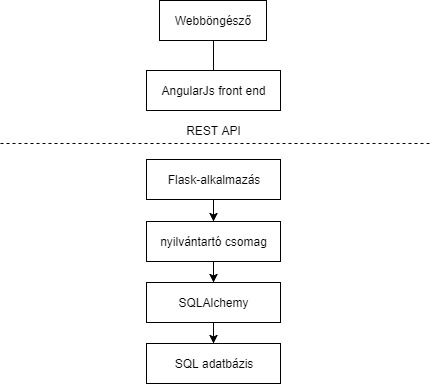
\includegraphics[scale=0.8]{kepek/architecture.jpg}
\caption{A webalkalmazás architektúrája}
\label{fig:architecture}
\end{figure}

A felhasználó böngészőn keresztül tudja használni az alkalmazást. Az alkalmazás használója ilyenkor az AngularJs-sel kialakított úgy nevezett nézeteket látja. Kliens oldalon az Angular kontrollerjei végzik a kérések elküldését a szerver irányába, melyekre a szerver az adatok visszaküldésével válaszol. A kapott válaszokat szintén az kontrollerek dolgozzák fel. A felhasználói felületről és az Angularról az ötödik fejezetben fogok bővebben írni.

% TODO: Apróság, de a fejezetet itt is majd \ref-el kellene hivatkozni!

A szerver oldalon egy többrétegű struktúrát hoztam létre. Az alsó réteg az adatbázis, ami egy SQLite alapú relációs adatbázis, amelyhez a keretrendszer SQLAlchemy ORM-en keresztül csatlakozik, tehát a lekérdezéseket az SQLAlchemy-vel végzem. Az SQL adatbázist a 4. fejezetben fogom részletesebben taglalni.

A klienstől érkező kérések feldolgozására az alkalmazás a Flask webes mikro keretrendszert használja. A flaskos réteg http válaszokat küld a kliensnek, melyeben az adatok JSON formátumúak. A flaskos réteg és az alsóbb rétegek között van egy közbenső réteg, az általam készített nyilvántartó csomag. A nyilvántartó csomagban lévő metódusok végzik a lekérdezéseket, ezeket a metódusokat hívom meg a flaskos rétegben. A közbenső réteg bevezetésére a későbbi továbbfejlesztési lehetőségek miatt volt szükség. A flask és a nyilvántartó csomag bemutatására a hetedik fejezben fog sor kerülni.
